% Created 2024-04-29 Mon 05:03
% Intended LaTeX compiler: pdflatex
\documentclass[tiny]{beamer}
\usepackage[utf8]{inputenc}
\usepackage[T1]{fontenc}
\usepackage{graphicx}
\usepackage{longtable}
\usepackage{wrapfig}
\usepackage{rotating}
\usepackage[normalem]{ulem}
\usepackage{amsmath}
\usepackage{amssymb}
\usepackage{capt-of}
\usepackage{hyperref}
\usepackage{minted}
\usepackage[french]{babel}
\usepackage[titles]{tocloft}
\usepackage{listings}
\definecolor{UBCblue}{rgb}{0.04706, 0.13725, 0.26667} % UBC Blue (primary)
\usecolortheme[named=UBCblue]{structure}
\usetheme{default}
\usecolortheme{beaver}
\usefonttheme{default}
\useinnertheme[shadow]{rounded}
\useoutertheme{infolines}
\author{Laurent Siksous}
\date{\today}
\title{Manul}
\subtitle{Renforcer l'Apprentissage de Hadoop avec des Environnements Pratiques}
\logo{
\includegraphics[height=0.9cm,keepaspectratio]{../../media/jems.png}\vspace{1040pt}}
\titlegraphic{
\includegraphics[width=50]{../../media/logo.png}}
\hypersetup{
 pdfauthor={Laurent Siksous},
 pdftitle={Manul},
 pdfkeywords={},
 pdfsubject={},
 pdfcreator={Emacs 29.1 (Org mode 9.6.6)}, 
 pdflang={French}}
\begin{document}

\maketitle
\begin{frame}{Outline}
\tableofcontents
\end{frame}

\section{Introduction}
\label{sec:orgb06cd09}

\begin{frame}[label={sec:org8967219}]{Introduction}
\begin{center}

\includegraphics[width=5cm]{../../media/manul.jpg}
\end{center}

\begin{quote}
"Embrassez la curiosité, explorez sans relâche, et laissez vos instincts vous
guider comme le Manul agile à travers les paysages accidentés de la
connaissance."
\end{quote}
\end{frame}

\begin{frame}[label={sec:org4617101}]{Aperçu du Projet}
\begin{itemize}
\item L'objectif de notre projet est de faciliter la création d'environnements
d'apprentissage pour l'enseignement des cours sur le Big Data.

\item Ces cours sont conçus pour fournir aux étudiants une expérience pratique de
travail avec les distributions Hadoop, y compris OSS, Cloudera et MapR.

\item Notre boîte à outils offre un déploiement facile de ces distributions
Hadoop en utilisant diverses méthodes, permettant aux étudiants d'explorer
différentes techniques de déploiement et de gestion de la configuration.

\item Cognitive Science:  \href{https://www.youtube.com/watch?v=v4oYOjVDgo0}{étapes du développement}
\end{itemize}
\end{frame}

\section{Contexte}
\label{sec:orgc08833c}

\begin{frame}[label={sec:orgd940601}]{Présentation de Datascientest}
Datascientest, une entreprise spécialisée dans l'enseignement des technologies
Big Data.

\begin{center}
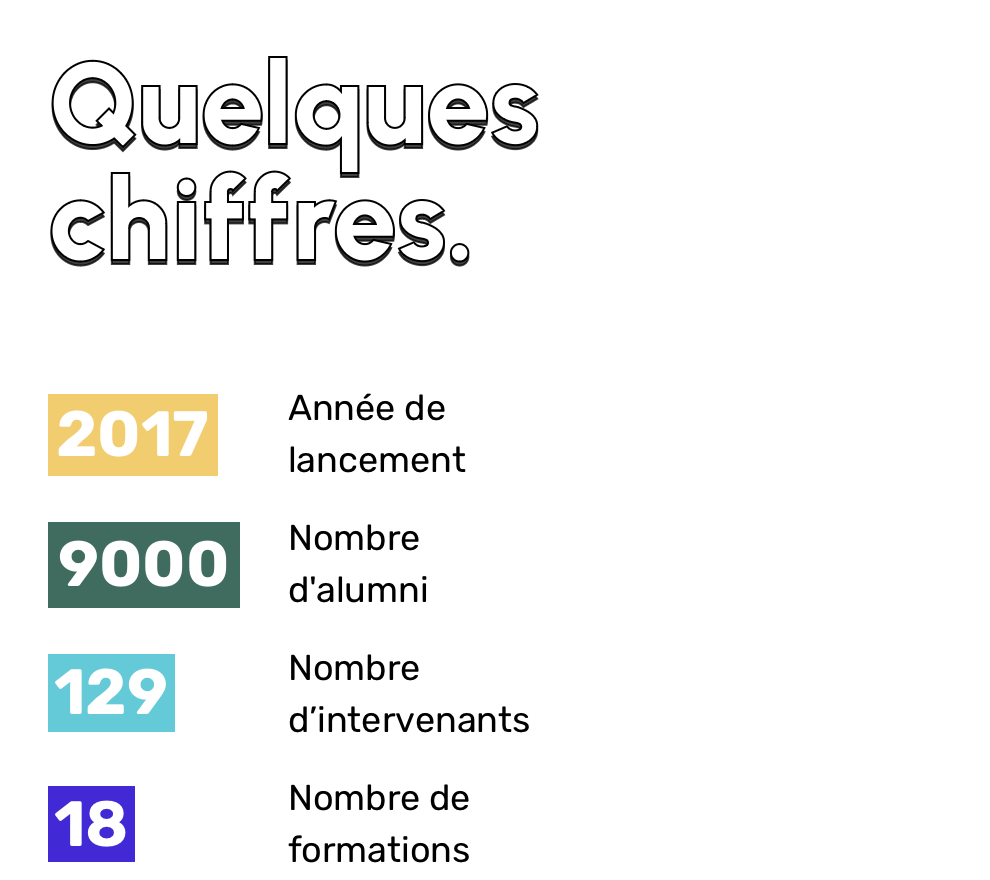
\includegraphics[width=5cm]{../../media/dst.png}
\end{center}
\end{frame}


\begin{frame}[label={sec:org4f4ebf1}]{Curriculum Hadoop}
\begin{center}
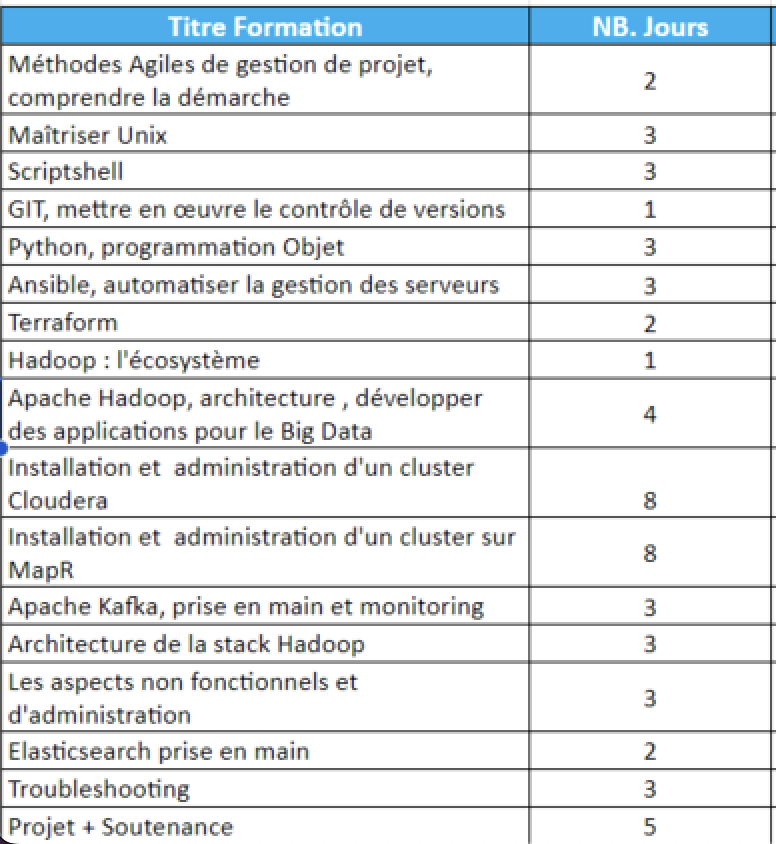
\includegraphics[width=5cm]{../../media/curriculum.png}
\end{center}
\end{frame}

\section{Problématique}
\label{sec:org6eda196}

\begin{frame}[allowframebreaks, labels=]{Problématique}
\begin{itemize}
\item \alert{Disparité des Environnements :} Chaque cours du curriculum utilise des
environnements Hadoop différents, ce qui entraîne une disparité et une
fragmentation des ressources et des outils pédagogiques.
\item \alert{Perte de Temps :} La configuration et la gestion manuelles des
environnements Hadoop pour chaque cours entraînent une perte de temps
significative pour les formateurs et les étudiants, limitant ainsi leur
capacité à se concentrer sur l'apprentissage des concepts essentiels.
\item \alert{Croyance dans l'Obsolescence de la Distribution MapR :} Malgré le support et
l'efficience de la documentation fournie par HPE Ezmeral Data Fabric,
Datascientest perçoit la distribution MapR comme étant en voie
d'obsolescence, ce qui soulève des préoccupations quant à la pertinence de
son inclusion dans le curriculum.
\item \alert{Raréfaction des Compétences MapR :} Avec la raréfaction des compétences MapR
sur le marché, il est devenu difficile de trouver des formateurs qualifiés
pour enseigner aux étudiants.
\item \alert{Demande Persistante des Clients :} Toutefois, la demande persistante des
clients de Datascientest pour des cours sur MapR nécessite une solution qui
puisse répondre à ces besoins tout en tenant compte des préoccupations
concernant l'obsolescence perçue de la distribution.
\end{itemize}

Datascientest a besoin d'une solution qui simplifie et standardise le
processus de déploiement des environnements Hadoop, tout en offrant une
expérience pratique et uniforme à ses étudiants.
\end{frame}


\section{Solution}
\label{sec:org76cf1c0}

\begin{frame}[label={sec:org973f791}]{Architecture}
\begin{center}
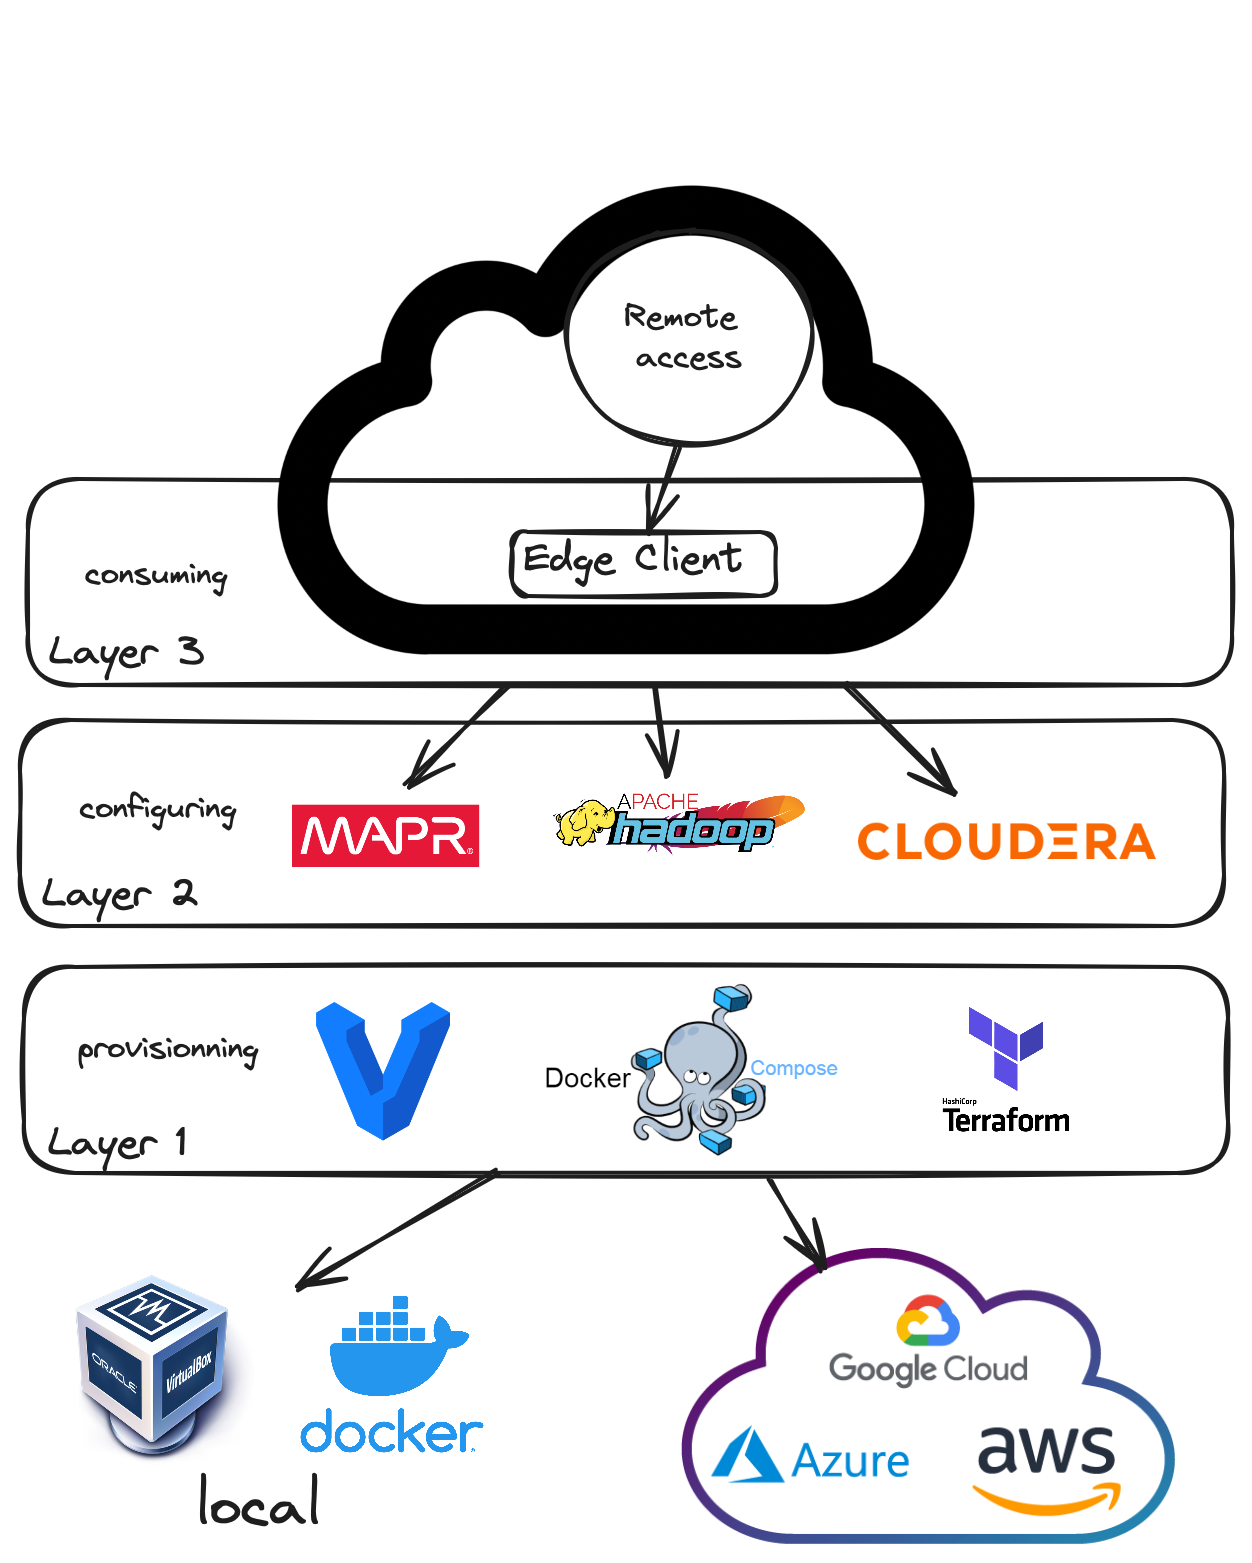
\includegraphics[width=5cm]{../../media/archi.png}
\end{center}
\end{frame}

\begin{frame}[allowframebreaks, labels=]{Fonctionnalités de la Boîte à Outils}
\begin{itemize}
\item \alert{Distributions Hadoop:} Notre boîte à outils prend en charge le déploiement
de trois principales distributions Hadoop : OSS, Cloudera et MapR. Cette
variété permet aux étudiants de se familiariser avec différentes
plateformes Hadoop et de comprendre leurs fonctionnalités et capacités
uniques.
\item \alert{Méthodes de Déploiement:} Nous proposons plusieurs méthodes de déploiement
pour répondre aux préférences et aux scénarios d'apprentissage différents :
\begin{itemize}
\item \alert{Docker:} Les étudiants peuvent déployer des environnements Hadoop à l'aide
de conteneurs Docker, offrant une solution légère et portable.
\item \alert{Vagrant:} Des environnements virtuels peuvent être créés à l'aide de
Vagrant, permettant aux étudiants de configurer des clusters Hadoop sur
leurs machines locales facilement.
\item \alert{Terraform:} Les enthousiastes de l'Infrastructure as Code (IaC) peuvent
utiliser Terraform pour provisionner des clusters Hadoop sur des
plates-formes cloud ou des fournisseurs de virtualisation.
\item \alert{Ansible:} Surtout axée sur Ansible, notre boîte à outils met l'accent sur
les techniques de gestion de configuration, permettant aux étudiants
d'automatiser la configuration et la gestion des environnements Hadoop.
\end{itemize}
\item \alert{Curriculum Intégré:} Les étudiants acquièrent une expérience pratique dans
le déploiement et la gestion de clusters Hadoop à l'aide d'outils standard
de l'industrie tels que Docker, Vagrant, Terraform et Ansible.
\end{itemize}
\end{frame}




\section{Démonstration}
\label{sec:orgb60db12}

\begin{frame}[label={sec:org90675cd}]{Démonstration}
\begin{itemize}
\item \url{https://github.com/lsiksous/manul}
\end{itemize}

\begin{center}
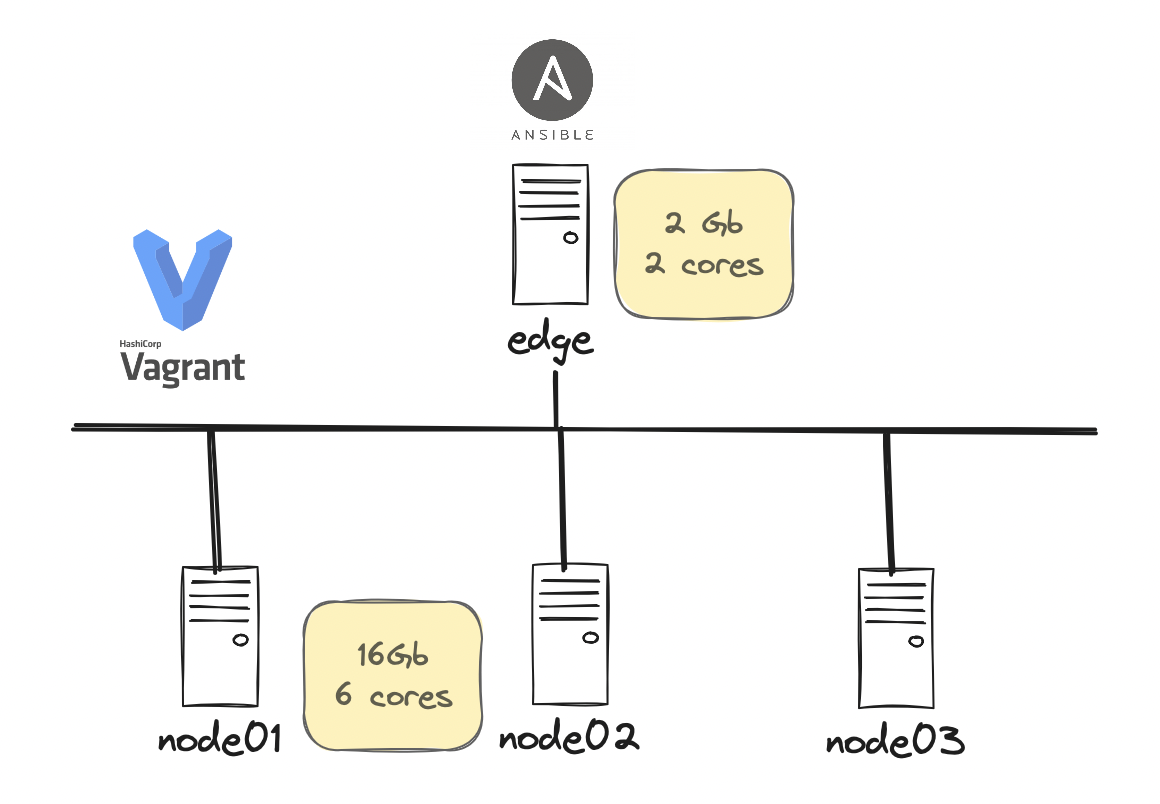
\includegraphics[width=5cm]{../../media/topo.png}
\end{center}
\end{frame}


\section{Références}
\label{sec:org09caa15}
\listoffigures

\bibliographystyle{unsrt}
\bibliography{references}
\end{document}